\documentclass[conference]{IEEEtran}
\usepackage{amsmath,amssymb}
\usepackage{graphicx}
\usepackage{booktabs}
\usepackage{tabularx}
\usepackage{cite}
\usepackage{url}
\usepackage{microtype}
\usepackage[T1]{fontenc}
\usepackage[utf8]{inputenc}
\graphicspath{{figures/}}

\begin{document}

\title{TRIAD: An Auditable Finite-Plan Receiver for Human-to-Robot Handover\\
\large Implementation, attribution and measured limits, with a robot-to-robot test setup}

\author{\IEEEauthorblockN{Hamidreza (Harry) J. Azari, Mourad Benoussaad, Wael Suleiman, Wiem Bel Hedi}
\IEEEauthorblockA{Author order, affiliations and venue to be confirmed.\\Manuscript of 24 September 2026, superseding the drafts of 3, 7 and 10 September 2026.}}

\maketitle

\begin{abstract}
TRIAD is a receiver-side controller for human-to-robot handover on a Kinova Gen3 arm with a Robotiq 2F-85 gripper, implemented on mc\_rtc. From one frozen planning state it enumerates a bounded bank of complete plans over event time, grasp and route (14 $\times$ 32 $\times$ 17 = 7616 before pruning), certifies each plan against modelled hard feasibility through acquisition and retreat, re-applies a timing admission rule at selection time, commits once and executes. This paper documents the implementation and, unlike the drafts that preceded it, does not present the decision structure as new: the timing rule is earliest-feasible rendezvous, the grasp stage is a reachability-screened funnel, and both are attributed to prior work. We report what instrumenting the system showed. In the original giver model the event time is imposed rather than predicted. Off-line replay shows that the exhaustive selection reduces to earliest admissible event time followed by the best grasp and route in 12 of 16 searches, and that four of five reach-certified grasps are later rejected at closure or retreat. A later variant that adds a predictive interception solver and a directional authority filter, compared against matched baselines on an identical plant, completed 6 of 12 scenarios against 11 of 12 for a plain predictive baseline. The evidence consists of four reference scenarios, a perception-latency sweep in which compensation extends completion from 0.22 s to 0.30 s of delay, an exact-serial performance measurement, the matched comparison, and a robot-to-robot test setup in which a second Gen3 presents the object: the full two-arm handover completes in simulation, and on hardware in July 2026 the giver arm executed its presentation alone while the combined run reached the receiver's committed reach before failing. No handover has been completed on hardware. Every number is regenerated from the public repository.
\end{abstract}

\section{Introduction}\label{sec:intro}
A robot that receives an object from a human must settle when the exchange will happen, how it will hold the object and along which path it will get there. TRIAD represents that decision as one finite object $\xi = (\tau, g, r)$, generates a bounded bank of complete candidates from one frozen planning state, rejects those that fail modelled feasibility checks through acquisition and retreat, ranks the survivors, re-checks timing admission against the controller clock, and commits exactly once.

Earlier drafts of this paper claimed the joint enumeration itself as the contribution. A source-level audit of 13 September 2026 and the repository's own instrumentation withdrew that claim: the timing rule reduces to earliest-feasible rendezvous, which Croft, Fenton and Benhabib \cite{croft98} and Huji\'c et al. \cite{hujic98} formulated in 1998; the grasp stage is the reachability-screened, cheap-to-exact funnel of Akinola et al. \cite{akinola21}; and the finite-time search over a predicted object trajectory is the pattern of Menon et al. \cite{menon14}, Salehian et al. \cite{salehian16} and Islam et al. \cite{islam20}. This version therefore makes a different, smaller claim.

\textbf{What this paper contributes.}
\begin{enumerate}
\item A complete, reproducible implementation of a finite-plan receiver on mc\_rtc, with its decision structure written down and each element attributed to the work it comes from (Section~\ref{sec:related}).
\item The measured limits of that structure on its own evidence: the event time is imposed in the original giver model, the exhaustive selection is dominated by earliest admissible timing, the seven-term cost was replaced by a lexicographic rule after off-line replay, and acquisition requires the object to be at rest (Section~\ref{sec:limits}).
\item A matched comparison in which the later, more elaborate variant loses to a plain predictive baseline (Section~\ref{sec:lite}).
\item A robot-to-robot test setup, a second Gen3 acting as the giver, integrated into the controller and verified in simulation, with the hardware status of July 2026 stated exactly (Section~\ref{sec:two}).
\end{enumerate}
No claim of a new decision method, of a control-performance gap, or of a hardware-validated handover is made.

\section{Related Work and Attribution}\label{sec:related}
\textbf{Interception timing.} Choosing the rendezvous instant as the earliest time at which the robot can reach the predicted object pose is the rendezvous-point selection of Croft, Fenton and Benhabib \cite{croft98} and the interception strategy of Huji\'c et al. \cite{hujic98}. Menon et al. \cite{menon14} pick the first forward time sample at which a bounded-velocity time of flight plus grasp time fits before the object arrives; Salehian et al. \cite{salehian16} take the first time at which the object enters the reachable set; Islam et al. \cite{islam20} plan for the pose projected forward by a fixed computation bound and replan with a commit cutoff. TRIAD's timing admission (Section~\ref{sec:method}) is a discretised instance of the same rule.

\textbf{Grasp selection under motion.} Akinola et al. \cite{akinola21} rank a fixed grasp database by precomputed reachability and motion awareness before exact inverse kinematics; Yang et al. \cite{yang21} refine a temporally consistent grasp set and resample when it is depleted. TRIAD's grasp stage is a cheap-ranking, bounded-exact-IK, first-success funnel of that kind.

\textbf{Handover controllers.} Yang et al. \cite{yang22} solve the receiver's motion with model predictive control over a goal set that couples grasp choice and motion; Oelerich et al. \cite{oelerich24} make progress along a path explicit in a path-following MPC; Djeha et al. \cite{djeha22} express handover constraints inside a task-space quadratic programme, which is also the execution layer TRIAD uses. Ortenzi et al. \cite{ortenzi21} review the field and identify the physical exchange as under-studied; Mason and MacKenzie \cite{mason05} measured the human--human transfer that these controllers imitate.

\textbf{What is left to TRIAD.} The combination is an implementation choice: a finite, inspectable plan set with a certification stage that models closure and retreat before commitment, on a task-space QP executor. The earlier drafts' Table~I, which marked the compared methods as lacking a ``finite complete-plan triple'', is withdrawn; explicitness of the plan is a property of the implementation, not a claim against those methods.

\section{The System}\label{sec:method}
\subsection{Platform and plant}
The receiver is a 7-DoF Kinova Gen3 with a Robotiq 2F-85 gripper, controlled by an mc\_rtc finite-state controller at 1 kHz. The object is the CALL two-handled body (0.346 kg, handles at $\pm$86.9 mm from the centre of mass). All reported evidence is simulation: the object pose is simulation truth, the transfer force is a virtual spring, and mc\_rtc runs without state feedback, so the controlled state is the control model. Fig.~\ref{fig:arch} shows the four layers.

\begin{figure}[t]\centering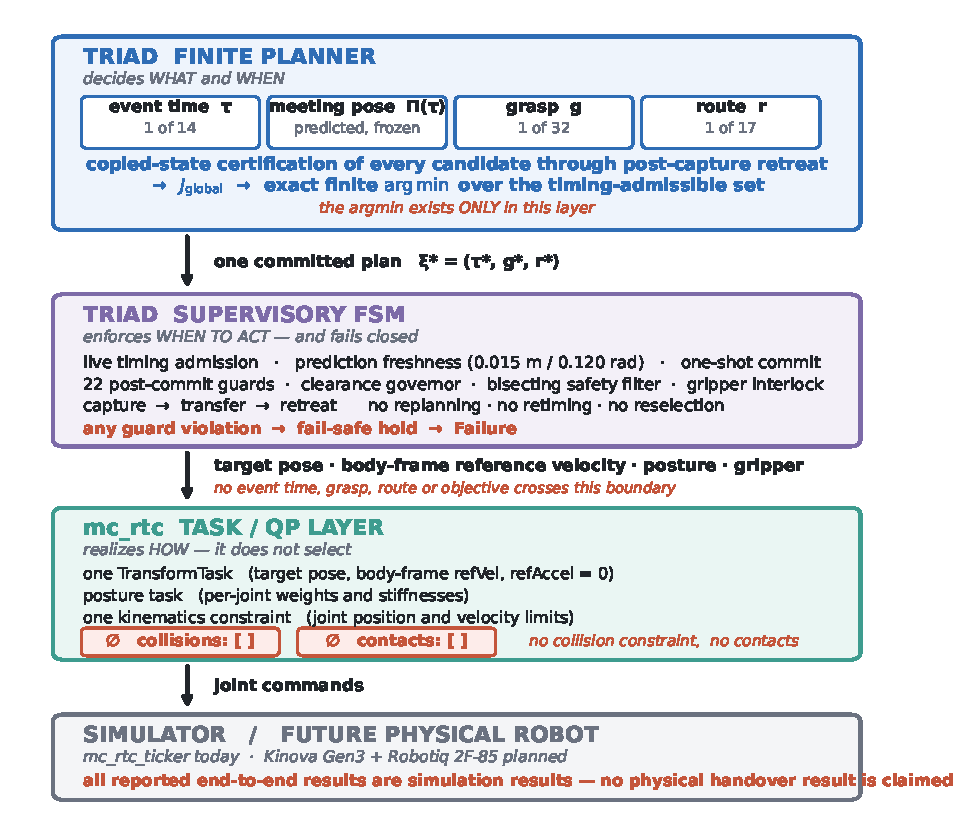
\includegraphics[width=0.98\columnwidth]{F01_architecture_four_layer.pdf}
\caption{Planner and execution architecture. TRIAD selects event time, grasp and route and emits one committed task-space plan; mc\_rtc's QP layer tracks it.}\label{fig:arch}\end{figure}

\subsection{The finite bank}
From a frozen snapshot at epoch $t_0$ the planner forms 14 event leads (1.80 to 8.00 s), 32 grasps (16 angles about the handle axis, two sign conventions) and 17 routes (direct plus 8 directions at two ring radii, 0.08 and 0.14 m); the pre-pruning product is 7616 (Fig.~\ref{fig:bank}). Object motion is propagated as a constant twist with a prescribed quintic stop; no covariance is maintained.

\begin{figure}[t]\centering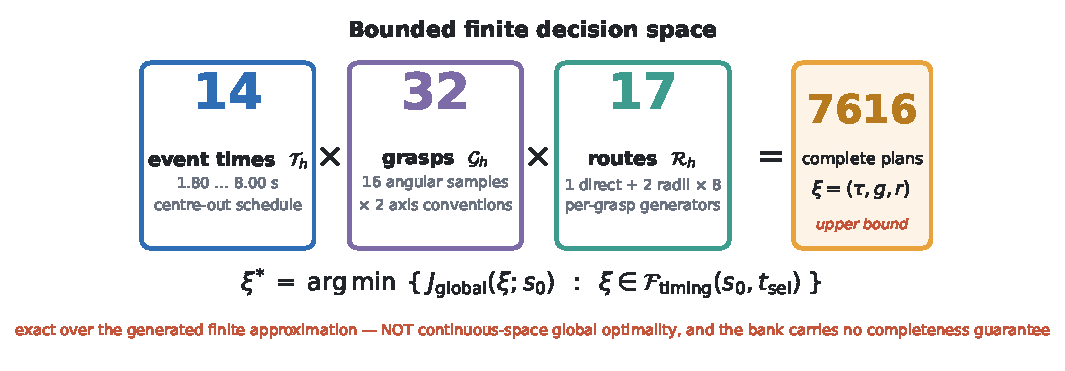
\includegraphics[width=0.98\columnwidth]{F05_finite_bank.pdf}
\caption{The bounded finite decision space, $14\times32\times17$.}\label{fig:bank}\end{figure}

\subsection{Certification, ranking and admission}
Every candidate is previewed by damped least-squares inverse kinematics on a copied robot state (step 0.020 s, damping 0.040, 25 swept poses per commanded segment) through reach, insertion, closure and retreat, with hard and soft clearance thresholds of 0.020 and 0.080 m. Survivors are ranked by a seven-term weighted cost referred to a common temporal origin; the weights (0.421, 0.105, 0.105, 0.158, 0.084, 0.074, 0.053) are frozen engineering preferences with no sensitivity study. The timing rule admits a plan only if the remaining lead exceeds a safe commit margin (1.6 s) and the predicted reach duration plus 0.050 s fits before the event. It is re-applied with the controller clock at selection, and a prediction-consistency gate of 0.015 m and 0.12 rad is checked at commitment (Fig.~\ref{fig:pipeline}). Exactly one plan is committed and executed without replanning. The search runs on a background worker; the control thread submits one generation and polls without blocking.

\begin{figure}[t]\centering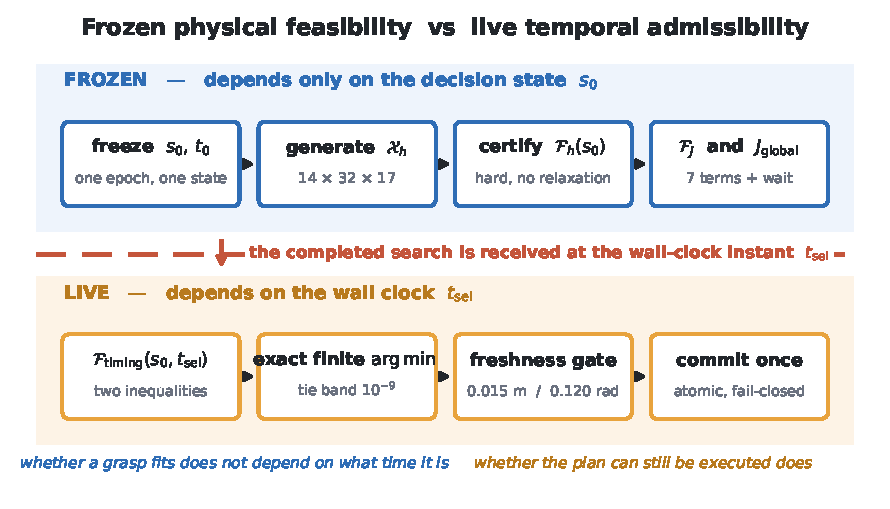
\includegraphics[width=0.98\columnwidth]{F06_frozen_live_pipeline.pdf}
\caption{Frozen-state certification versus live timing admission.}\label{fig:pipeline}\end{figure}

\subsection{Later variants}
A receding variant (V2) replaces the single frozen search by a supervisor that re-certifies the active plan, cancels and restarts the search when the object estimate changes, and commits at a terminal boundary; it uses a robot-independent scripted giver. A further variant (TRIAD-lite) adds a sampled earliest-feasible rendezvous solver over a 530-hypothesis grasp family and a directional velocity-authority filter $\kappa$ computed from the QP's joint-velocity box. All variants share the acquisition interface: closure is gated on the object being at rest (4 mm/s).

\section{What the Instrumentation Showed}\label{sec:limits}
\textbf{The event time is imposed in the original giver model.} In the V1 configuration the simulated giver follows the committed presentation time after commitment. The event time is therefore not a prediction that the world may or may not honour; it is a schedule the robot sets. The V2 independent giver removes this, at the cost of the moving-epoch search (2.9 to 3.9 s) exceeding the constant-velocity window (3.67 s).

\textbf{Selection is dominated by timing.} Off-line replay of logged certifications with a validated selector replica shows that the zero-latency exhaustive argmin equals ``earliest admissible $\tau$, then best $(g,r)$'' in 12 of 16 searches; as executed, the search latency changes the chosen $\tau$ in every moving scenario. In TRIAD-lite the $\tau$ axis is an ascending first-feasible scan, and with the rest gate active it has size one.

\textbf{The seven-term cost did not survive replay.} Its regret reached 1.38 s and its winner flipped under weight perturbation in up to 21 of 40 cases; it was replaced by a lexicographic rule (completion, then clearance, then effort). The lateral-low ``route required'' finding was a reach-duration artefact (28 of 34 cases rescued by a 1.2$\times$ time stretch).

\textbf{Reach certification is a weak filter.} 78 to 81 \% of reach-feasible grasps are rejected at closure or retreat; reach-only selection picks a later-rejected action in 9 of 12 searches (Fig.~\ref{fig:funnel}).

\textbf{Prediction validity is short.} The 15 mm validity horizon while the object moves is 0.10 to 0.65 s; plans adopted while moving realised up to 313 mm of error.

\begin{figure}[t]\centering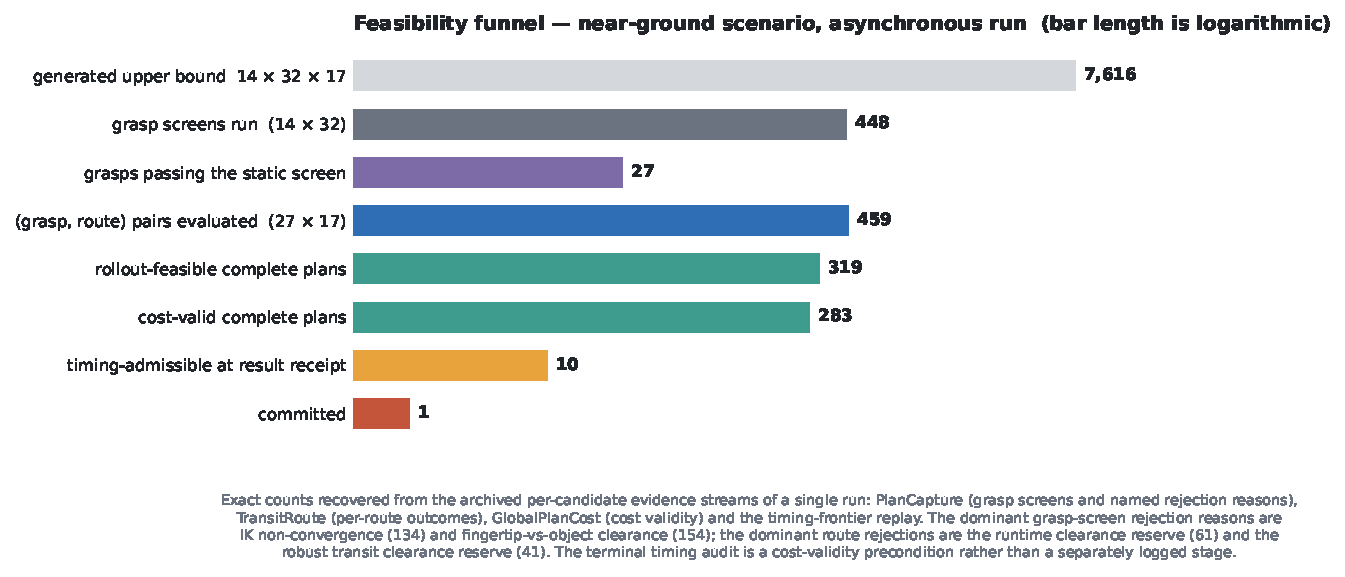
\includegraphics[width=0.98\columnwidth]{F13_feasibility_funnel.pdf}
\caption{Feasibility funnel for the near-ground scenario with the archived counts.}\label{fig:funnel}\end{figure}

\section{Evaluation}\label{sec:eval}
\subsection{Reference scenarios}
Four moving-object scenarios provide the reference winners of the frozen selector (Table~\ref{tab:ref}). They are reference runs, not a controlled comparison.

\begin{table}[t]\caption{Reference scenarios: committed plan and completion (simulation).}\label{tab:ref}\centering\small
\setlength{\tabcolsep}{4pt}\begin{tabular}{lcccc}\toprule
scenario & $\tau^*$ (s) & route & $J_{\mathrm{glob}}$ & compl. pred./act. (s)\\\midrule
near-ground & 4.600 & ring 80 mm & 0.823 & 9.80 / 8.47\\
longitudinal & 3.700 & direct & 0.687 & 8.70 / 7.29\\
lateral-low & 4.150 & direct & 0.701 & 8.80 / 7.44\\
diagonal & 4.600 & ring 140 mm & 0.685 & 9.62 / 8.22\\\bottomrule
\end{tabular}\end{table}

\subsection{Perception latency}
A timestamped delay is injected into the object-pose measurement and either propagated by its measured age (compensated) or treated as current. Both modes complete at 0.10 and 0.22 s of delay. At 0.30 s only the compensated mode completes (four of four repeats against zero of four). From 0.40 s both modes commit and fail in execution; at 0.60 s the compensated mode is rejected before commitment by the freshness gate and the uncompensated mode cannot classify the object (displacement 0.0241 m below the 0.0250 m moving threshold while the estimated speed exceeds the static threshold). Compensation therefore extends the usable delay from 0.22 s to 0.30 s in this configuration, no further.

\subsection{Exact-serial performance}
Restructuring the serial search reduced the state-scoped wall time from 4.349 to 3.972 s, 3.315 to 3.072 s, 3.393 to 3.162 s and 2.797 to 2.620 s over the four scenarios (6.3 to 8.7 \%), with a collision oracle of 8\,168\,732 comparisons and zero mismatches against the reference.

\subsection{Matched comparison of the later variant}\label{sec:lite}
Four selectors were run over four scenarios with three near-deterministic repeats each, on an identical plant, an identical grasp pool and one evaluator (Table~\ref{tab:lite}). The proposed variant with the hard authority filter is the second worst. An earlier campaign had reported FULL at 12 of 12 and B1 at 9 of 12; that came from a rollout defect on replans from a moving arm that inflated the demand signal the filter consumes. Both campaigns are archived. The predictive variants meet the grasp pose 1.5 to 3 mm from the target and up to 1.6 s before the giver stops, but acquisition still waits for rest, so the difference between B0 and B1 concerns reaching a rendezvous, not acquiring a moving object, and the B0 baseline differs from B1 in more than the predictive term.

\begin{table}[t]\caption{Matched comparison (TRIAD-lite, simulation, 12 runs per selector).}\label{tab:lite}\centering\small
\begin{tabular}{llc}\toprule
selector & description & completions\\\midrule
B0 & reactive baseline & 5/12\\
B1 & plain predictive baseline & 11/12\\
B2 & capability tie-break & 10/12\\
FULL & joint selection with the authority filter & 6/12\\\bottomrule
\end{tabular}\end{table}

\section{Robot-to-Robot Test Setup}\label{sec:two}
\subsection{Setup}
To exercise the receiver without a human, a second Kinova Gen3 without a gripper role (Robot B, base at $[1.35, 0, 0]$ m, yaw $\pi$) presents the object along a fixed world-frame trajectory while Robot A receives (Fig.~\ref{fig:two}). Robot B is coordinated inside the controller by a giver module: it prepositions to the scenario start, settles, waits for Robot A's object observation to begin, executes the presentation (0.08 m/s along $-x$, from $[0.92,0,0.55]$ to $[0.55,0,0.55]$ m, 0.85 s deceleration), settles at the terminal gate and holds; the object is rigidly coupled to Robot B's tool until Robot A acquires it. Robot A's FSM is unchanged. An alternative runs Robot B from a second computer with no communication, from a fixed start and a single trigger.

\begin{figure}[t]\centering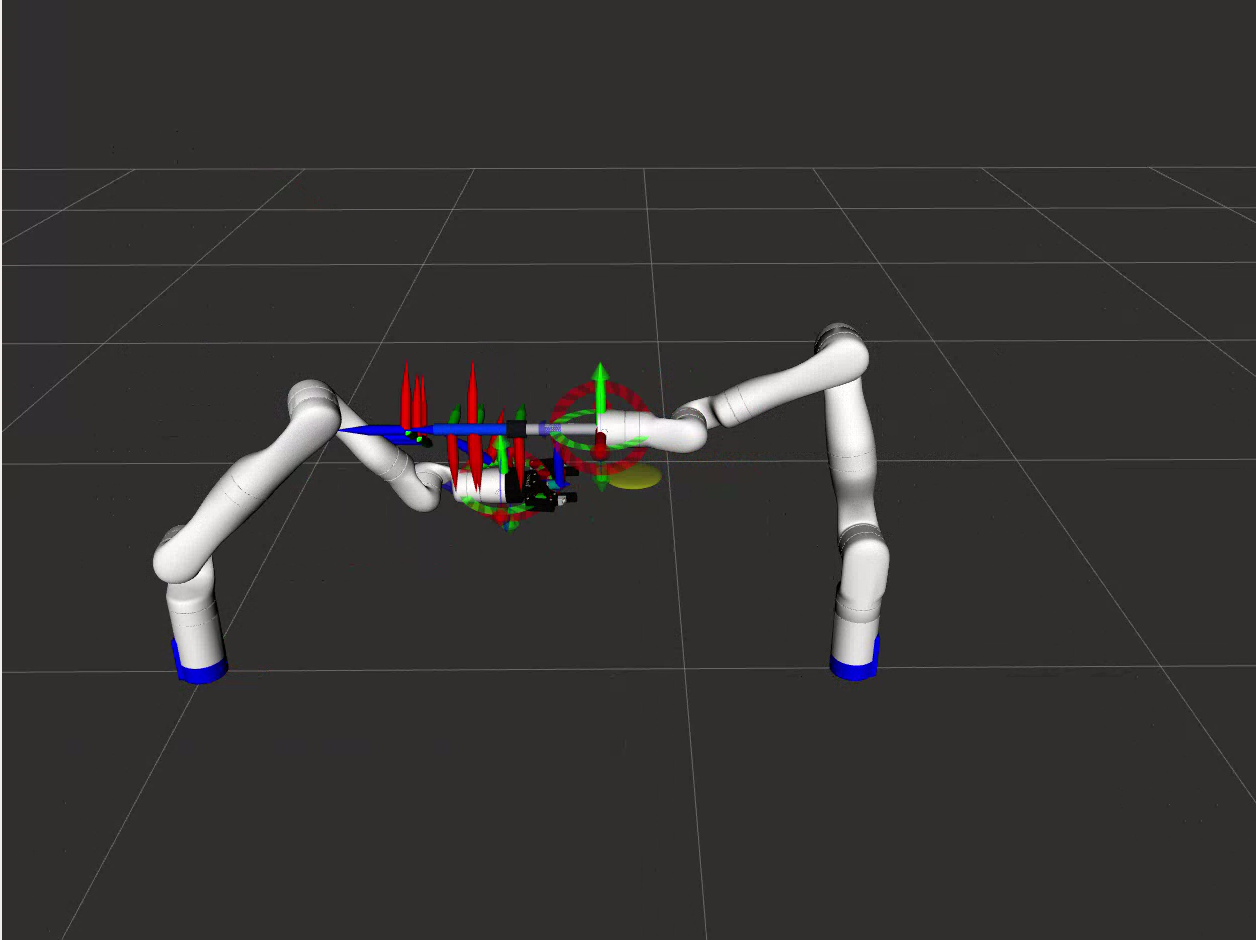
\includegraphics[width=0.98\columnwidth]{two_robot_sim.png}
\caption{Robot B (right) presenting the object to Robot A (left) in the two-arm simulation, 18 July 2026.}\label{fig:two}\end{figure}

\subsection{Simulation}
On 24 September 2026, with the giver module ported onto the final code, the full two-arm handover completed in mc\_rtc's simulation: Robot B was at rest at the start at 2.7 s, executed from 8.1 s, and held from 13.4 s; Robot A entered observation at 7.8 s, committed at 12.1 s, captured at 15.7 s, retreated at 19.4 s and reported completion at 19.9 s (execution 7.5 s against 8.9 s predicted). The single-robot scenario completes on the same build, and so does a run with the second robot loaded and the giver disabled.

\subsection{Hardware status, July 2026}
Both arms were driven from one computer through per-robot Kortex bridges on 17 and 18 July 2026; the logs contain the second arm's motor currents and driver temperatures, which only a physical robot produces. Robot B executed its presentation alone on hardware through all six phases (17 July, 22:30). The combined run of 18 July (00:51) reached Robot A's committed reach and failed before capture. Robot A's gripper had been commissioned on hardware on 15 and 16 July with a measured closure calibration. No hardware run reached the capture state, the transfer force source was virtual in every hardware run, and no run of the final code has been made on hardware. The procedure, the receiver's hardware switches and the log inventory are in the repository.

\section{Discussion and Limitations}\label{sec:disc}
The evidence supports an implementation claim and nothing stronger. Three limits are structural. First, acquisition requires the object to stop, so no variant acquires a moving object; the predictive machinery serves the approach only. Second, no control-performance gap is established: the one matched comparison is lost by the more elaborate variant, and the reference scenarios have no external baseline. Third, everything is simulation with virtual force; the two-robot setup makes hardware testing possible without a human but has not yet produced a completed handover. The bank is an engineering discretisation with no resolution study; the cost weights were replaced rather than justified. What is reusable is the plant, the certification stage that models closure and retreat, the evaluation tooling, and a test setup on which a receiver can be exercised repeatably.

\section{Reproducibility}\label{sec:repro}
The controller, the configuration, the evidence records, the two-robot extension and the scripts that regenerate every number in this paper are in the TRIAD repository (branch \texttt{triad/two-robot-2026-09-24}, tag \texttt{triad-final-2026-09-24}). The unit tests and documentation-claim guards run in continuous integration; the two-arm simulation runs from a build tree with one script.

\section{Conclusion}\label{sec:conc}
TRIAD is an auditable finite-plan receiver whose decision structure is prior art and whose own instrumentation shows that timing dominates selection, that the original giver model imposes the event time, and that a more elaborate variant loses to a plain predictive baseline. Its value is the implementation, the attribution, the measured limits, and a robot-to-robot setup on which the next question can be tested on hardware.

\begin{thebibliography}{12}
\bibitem{croft98} E. A. Croft, R. G. Fenton, and B. Benhabib, ``Optimal rendezvous-point selection for robotic interception of moving objects,'' \emph{IEEE Trans. Syst., Man, Cybern. B}, vol. 28, no. 2, 1998. [Bibliographic details to be verified before submission.]
\bibitem{hujic98} D. Huji\'c, E. A. Croft, G. Zak, R. G. Fenton, J. K. Mills, and B. Benhabib, ``The robotic interception of moving objects in industrial settings: strategy development and experiment,'' \emph{IEEE/ASME Trans. Mechatronics}, vol. 3, no. 3, 1998. [Bibliographic details to be verified before submission.]
\bibitem{menon14} A. Menon, B. Cohen, and M. Likhachev, ``Motion planning for smooth pickup of moving objects,'' in \emph{Proc. IEEE ICRA}, 2014, pp. 453--460.
\bibitem{salehian16} S. S. Mirrazavi Salehian, N. Figueroa, and A. Billard, ``Coordinated multi-arm motion planning: reaching for moving objects in the face of uncertainty,'' in \emph{Proc. Robotics: Science and Systems}, 2016.
\bibitem{islam20} F. Islam, O. Salzman, A. Agarwal, and M. Likhachev, ``Provably constant-time planning and replanning for real-time grasping objects off a conveyor belt,'' in \emph{Proc. Robotics: Science and Systems}, 2020.
\bibitem{akinola21} I. Akinola, J. Xu, S. Song, and P. K. Allen, ``Dynamic grasping with reachability and motion awareness,'' in \emph{Proc. IEEE/RSJ IROS}, 2021.
\bibitem{yang21} W. Yang, C. Paxton, A. Mousavian, Y.-W. Chao, M. Cakmak, and D. Fox, ``Reactive human-to-robot handovers of arbitrary objects,'' in \emph{Proc. IEEE ICRA}, 2021.
\bibitem{yang22} W. Yang, B. Sundaralingam, C. Paxton, I. Akinola, Y.-W. Chao, M. Cakmak, and D. Fox, ``Model predictive control for fluid human-to-robot handovers,'' in \emph{Proc. IEEE ICRA}, 2022.
\bibitem{oelerich24} T. Oelerich, C. Hartl-Nesic, and A. Kugi, ``Model predictive trajectory planning for human-robot handovers,'' arXiv:2404.07505, 2024.
\bibitem{djeha22} M. Djeha et al., ``Human-robot handovers using task-space quadratic programming,'' in \emph{Proc. IEEE RO-MAN}, 2022.
\bibitem{ortenzi21} V. Ortenzi, A. Cosgun, T. Pardi, W. P. Chan, E. Croft, and D. Kuli\'c, ``Object handovers: a review for robotics,'' \emph{IEEE Trans. Robotics}, vol. 37, no. 6, 2021.
\bibitem{mason05} A. H. Mason and C. L. MacKenzie, ``Grip forces when passing an object to a partner,'' \emph{Exp. Brain Res.}, vol. 163, 2005.
\end{thebibliography}

\end{document}
